\section{Final unity structure}
In unity there has been create two scenes: StartMenu, and Main scene.
This section will give an overview of these two scenes, and show the game objects that has been used in this project.

\subsection{Start menu}
The start menu is the lobby and the game objects within the scene can be seen on \autoref{fig:startmenu-game-objects}.
The five main game objects are the \texttt{GameStateHandler}, \texttt{ConnectionHandler}, \texttt{EventSystem}, \texttt{Menu}, and the standard \texttt{Main Camera}.
\\
The \texttt{GameState} contains a simple script with GameState information such as Anchor positions, player positions and other different variables used when the game start.
It also contains another script \texttt{DontDestroy}, which ensures that the game object does not get destroyed when changing scene.
\\
\texttt{ConnectionHandler} contains the scripts \texttt{DontDestroy} and \texttt{TCPClient}.
The \texttt{TCPClient} receives the information from the host and adds the information received to the \texttt{GameState}.
\\
\texttt{Menu} has multiple game objects as children, which are used to specify how the UI should look.
Menu has also a script, which disables virtual reality in this scene.
The \texttt{ConnectButton} and \texttt{CancelConnection} uses an \texttt{OnClick} feature in unity, where it call as function to either connect or cancel the connection.
\\
The \texttt{EventSystem} supports sending events to objects based on input as clicks on button or typing in the text field.

\begin{figure}[H]
    \centering
    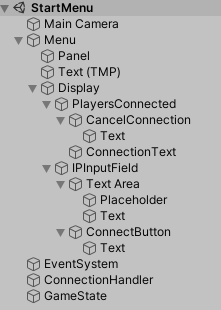
\includegraphics[width=0.4\linewidth]{figures/startmenu.PNG}
    \caption{The game objects in the start menu.}
    \label{fig:startmenu-game-objects}
\end{figure}

\subsection{Main scene}
The main scene is the game scene with the playing field.
The primary objects in main is \texttt{CLIENT}, \texttt{PlayingFieldContainer}, \texttt{Camera Rig} and \texttt{GvrEventSystem}.
These can be seen on \autoref{fig:main-game-objects}.
\\\\
The \texttt{CLIENT} contains the script \texttt{UDPClient}, which instantiates the UDP client and receives player and ball positions.
This script is previously described in \autoref{sec:receiving-the-information}.
\\
The \texttt{PlayingFieldContainer} only has \texttt{PlayingField} as a child and has the script \texttt{CameraFollow} attached.
This script ensures that the playing field is always in the center of the camera.
The \texttt{PlayingField} has two children, where one of them is the GoalZoneController, which is used to generate the playing field and make sure that the entire field is visible with the camera.
The other is the \texttt{Goalscore-UI}, which is used to display the current score of the game.
It has two script attached to the game object \texttt{FieldGenerator} and \texttt{PlayingFieldOffset}.
\texttt{FieldGenerator} creates the playing field from the coordinates coordinates in the \texttt{GameStateHandler}, which was instantiated in the lobby.
\texttt{PlayingFieldOffset} is used to change the center coordinate of the field, so that it has the same $x$ and $y$ position as the camera.

\begin{figure}[H]
    \centering
    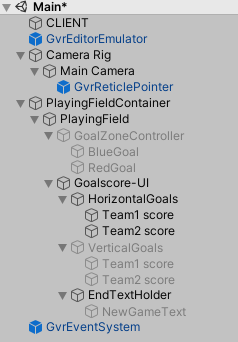
\includegraphics[width=0.4\linewidth]{figures/unity-main-gameobjects.PNG}
    \caption{The game objects in the main game scene.}
    \label{fig:main-game-objects}
\end{figure}

